\documentclass{article}

% Packages
\usepackage{fullpage}
\usepackage{graphicx}
\usepackage{verbatim}

% Macros
% INSERT HW NUM HERE
\newcommand{\HWNUM}{1}

\newcommand{\PI}[1]{\begin{scriptsize}\begin{verbatim}#1\end{verbatim}\end{scriptsize}}

\begin{document}

    % TITLE SECTION

    \begin{center}
        ************************************ \\
        EE/CS 119A Homework \HWNUM \\
        Edward Speer \\
        \today \\
        ************************************
    \end{center}

    % PROBLEMS
    \begin{enumerate}
    
        \item \textbf{Problem 1}: \emph{7-Segment Decimal Counter} \\
            
            Begin by creating the truth table for the 7-segment display. In this
            table, $x_1$ will represent a signal currently stored in the DFFs,
            and $x_2$ will represent desired next signal to be stored in the
            DFFs.

            \begin{center}
                \begin{tabular}{|c c c c c c c|c c c c c c c|}
                \hline
                $a_1$&$b_1$&$c_1$&$d_1$&$e_1$&$f_1$&$g_1$&
                $a_2$&$b_2$&$c_2$&$d_2$&$e_2$&$f_2$&$g_2$\\
                \hline
                1&1&1&1&1&1&0& 0&1&1&0&0&0&0\\
                0&1&1&0&0&0&0& 1&1&0&1&1&0&1\\
                1&1&0&1&1&0&1& 1&1&1&1&0&0&1\\
                1&1&1&1&0&0&1& 0&1&1&0&0&1&1\\
                0&1&1&0&0&1&1& 1&0&1&1&0&1&1\\
                1&0&1&1&0&1&1& 0&0&1&1&1&1&1\\
                0&0&1&1&1&1&1& 1&1&1&0&0&0&0\\
                1&1&1&1&1&1&1& 1&1&1&0&0&1&1\\
                1&1&1&0&0&1&1& 1&1&1&1&1&1&0\\
                \hline
                \end{tabular}
            \end{center}

            I then leveraged the Quine-McCluskey software that I wrote for HW2
            (attached) to write a script (also attached) that would generate the
            prime implicants table for each of the segments in the display. From
            the prime implicants table, the equations for each segment may be
            derived. To generate the equation for each signal, I combined the
            results from the prime implicants chart with the reset mechanism.
            For reset, I take the OR of all the segments that are on to display
            the number 0 with the RESET signal, and the AND of the only segment
            that's off in displaying 0 with the negation of the RESET signal.
            This way, when reset is high, the display will be forced to show 0.
            Call the reset signal $r$.

            For $a$:
            \begin{scriptsize}
            \begin{verbatim}
Signal: a
==============================================
| .....00 | x ||   ||   ||   || x ||   ||   |
----------------------------------------------
| ....0.0 | x ||   ||   ||   || x ||   ||   |
----------------------------------------------
| ....1.1 |   || x ||   || x ||   || x ||   |
----------------------------------------------
| ....10. |   || x ||   ||   ||   ||   ||   |
----------------------------------------------
| ...0... | x ||   || x ||   || x ||   || x |
----------------------------------------------
| ..0.... |   || x ||   ||   ||   ||   ||   |
----------------------------------------------
| .0..1.. |   ||   ||   || x ||   ||   ||   |
----------------------------------------------
| .1...11 |   ||   || x ||   ||   || x || x |
----------------------------------------------
| .1..01. |   ||   || x ||   ||   ||   || x |
----------------------------------------------
| 0...... | x ||   || x || x ||   ||   ||   |
----------------------------------------------
==============================================
            \end{verbatim}
            \end{scriptsize}
            From the prime implicants table, rows 3 and 5 form a minimal
            covering set for the minterms so that \fbox{$a = eg + d' + r$}
            \pagebreak

            For $b$:
            \begin{scriptsize}
            \begin{verbatim}
Signal: b
===================================================
| ......0 | x || x ||   ||   ||   || x ||   ||   |
---------------------------------------------------
| .....0. |   || x || x || x ||   || x ||   ||   |
---------------------------------------------------
| ....1.. | x ||   || x ||   || x ||   || x ||   |
---------------------------------------------------
| ..0.... |   ||   || x ||   ||   ||   ||   ||   |
---------------------------------------------------
| .1.1... | x ||   || x || x ||   ||   || x ||   |
---------------------------------------------------
| 0..1... |   ||   ||   ||   || x ||   ||   ||   |
---------------------------------------------------
| 00..... |   ||   ||   ||   || x ||   ||   ||   |
---------------------------------------------------
| 1..0... |   ||   ||   ||   ||   || x ||   || x |
---------------------------------------------------
| 11..... | x ||   || x || x ||   || x || x || x |
---------------------------------------------------
===================================================
            \end{verbatim}
            \end{scriptsize}
            There are many possible covering sets for $b$, but one using the
            fewest total signals would be rows 2, 3, and 9. This yields 
            \fbox{$b = ab + e + f' + r$}

            For $c$:
            \begin{scriptsize}
            \begin{verbatim}
Signal: c
========================================================
| ......1 |   || x || x || x || x || x ||   || x || x |
--------------------------------------------------------
| .....1. | x ||   ||   || x || x || x ||   || x || x |
--------------------------------------------------------
| ....1.. | x || x ||   ||   ||   || x ||   || x ||   |
--------------------------------------------------------
| ...1... | x || x || x ||   || x || x ||   || x ||   |
--------------------------------------------------------
| ..0.... |   || x ||   ||   ||   ||   ||   ||   ||   |
--------------------------------------------------------
| .0..... |   ||   ||   ||   || x || x ||   ||   ||   |
--------------------------------------------------------
| 1...... | x || x || x ||   || x ||   || x || x || x |
--------------------------------------------------------
========================================================
            \end{verbatim}
            \end{scriptsize}
            $c$ has a clear minimal covering set from rows 1 and 7, yielding 
            \fbox{$c = a + g + r$}
            \pagebreak

            for $d$:
            \begin{scriptsize}
            \begin{verbatim}
Signal: d
=========================================
| .....00 | x ||   ||   ||   || x ||   |
-----------------------------------------
| ....0.0 | x ||   ||   ||   || x ||   |
-----------------------------------------
| ....01. |   ||   || x || x ||   || x |
-----------------------------------------
| ....10. |   || x ||   ||   ||   ||   |
-----------------------------------------
| ...0... | x ||   || x ||   || x || x |
-----------------------------------------
| ..0.... |   || x ||   ||   ||   ||   |
-----------------------------------------
| .0..0.. |   ||   ||   || x ||   ||   |
-----------------------------------------
| 0.....0 | x ||   ||   ||   ||   ||   |
-----------------------------------------
| 0....0. | x ||   ||   ||   ||   ||   |
-----------------------------------------
| 0...0.. | x ||   || x ||   ||   ||   |
-----------------------------------------
| 01..... | x ||   || x ||   ||   ||   |
-----------------------------------------
| 10..... |   ||   ||   || x ||   ||   |
-----------------------------------------
=========================================
            \end{verbatim}
            \end{scriptsize}
            $d$ has many possible covering sets, but the one using the fewest
            total signals is rows 5, 6, and 12. This yields
            \fbox{$d = ab' + c' + d' + r$}

            for $e$:
            \begin{scriptsize}
            \begin{verbatim}
Signal: e
===============================
| .....00 | x ||   || x ||   |
-------------------------------
| ....0.0 | x ||   || x ||   |
-------------------------------
| ...0..0 | x ||   || x ||   |
-------------------------------
| ...0.0. | x ||   || x ||   |
-------------------------------
| ...101. |   || x ||   ||   |
-------------------------------
| .0..0.. |   || x ||   ||   |
-------------------------------
| 0.....0 | x ||   ||   ||   |
-------------------------------
| 0....0. | x ||   ||   ||   |
-------------------------------
| 1...01. |   || x ||   || x |
-------------------------------
| 1..0... |   ||   || x || x |
-------------------------------
| 10..... |   || x ||   ||   |
-------------------------------
===============================
            \end{verbatim}
            \end{scriptsize}
            $e$ has multiple possible covering sets, but I chose the one using
            rows 1 and 9. This yields \fbox{$e = f'g' + ae'f + r$}
            \pagebreak

            for $f$:
            \begin{scriptsize}
            \begin{verbatim}
Signal: f
=========================================
| ....0.1 | x || x || x ||   ||   || x |
-----------------------------------------
| ....01. |   || x || x ||   ||   || x |
-----------------------------------------
| ...0..1 |   || x ||   ||   ||   || x |
-----------------------------------------
| ...0.1. |   || x ||   ||   ||   || x |
-----------------------------------------
| ...10.. | x ||   || x ||   ||   ||   |
-----------------------------------------
| ..1..01 | x ||   ||   ||   ||   ||   |
-----------------------------------------
| ..11.0. | x ||   ||   ||   ||   ||   |
-----------------------------------------
| .0..0.. |   ||   || x ||   ||   ||   |
-----------------------------------------
| .1...11 |   || x ||   ||   || x || x |
-----------------------------------------
| .11...1 | x || x ||   ||   || x || x |
-----------------------------------------
| 01....1 |   || x ||   ||   ||   ||   |
-----------------------------------------
| 01...1. |   || x ||   ||   ||   ||   |
-----------------------------------------
| 1....00 |   ||   ||   || x ||   ||   |
-----------------------------------------
| 1....11 |   ||   || x ||   || x || x |
-----------------------------------------
| 1...0.. | x ||   || x || x ||   || x |
-----------------------------------------
| 1..0... |   ||   ||   || x ||   || x |
-----------------------------------------
| 1.1...1 | x ||   || x ||   || x || x |
-----------------------------------------
| 1.1..0. | x ||   ||   || x ||   ||   |
-----------------------------------------
| 10..... |   ||   || x ||   ||   ||   |
-----------------------------------------
=========================================
            \end{verbatim}
            \end{scriptsize}

            $f$ has several possible covering sets, but the one using the least 
            total signals is rows 15 and 9. This yields
            \fbox{$f = ae' + bcg + r$}
            \pagebreak

            for $g$:
            \begin{scriptsize}
            \begin{verbatim}
Signal: g
==============================================
| .....0. | x || x || x ||   ||   || x ||   |
----------------------------------------------
| ....0.0 | x ||   ||   ||   ||   || x ||   |
----------------------------------------------
| ...0..0 | x ||   ||   ||   ||   || x ||   |
----------------------------------------------
| ...10.. |   ||   || x ||   || x ||   ||   |
----------------------------------------------
| ..0.... |   || x ||   ||   ||   ||   ||   |
----------------------------------------------
| .0..0.. |   ||   ||   ||   || x ||   ||   |
----------------------------------------------
| .1..1.1 |   || x ||   ||   ||   ||   || x |
----------------------------------------------
| .1.1..1 |   || x || x ||   ||   ||   || x |
----------------------------------------------
| 0.....0 | x ||   ||   ||   ||   ||   ||   |
----------------------------------------------
| 0...0.. | x ||   ||   || x ||   ||   ||   |
----------------------------------------------
| 0..0... | x ||   ||   || x ||   ||   ||   |
----------------------------------------------
| 01..... | x ||   ||   || x ||   ||   ||   |
----------------------------------------------
| 1...1.1 |   || x ||   ||   ||   ||   || x |
----------------------------------------------
| 1..1..1 |   || x || x ||   || x ||   || x |
----------------------------------------------
| 10..... |   ||   ||   ||   || x ||   ||   |
----------------------------------------------
==============================================
            \end{verbatim}
            \end{scriptsize}
            $g$ has multiple possible covering sets, but the one using the least
            total signals is from rows 1, 14, and 12. This yields
            \fbox{$g = r'(a'b + adg + f')$}

            These equations are implemented in AND/OR/INVERT logic in the 
            following circuit:
            \begin{center}
                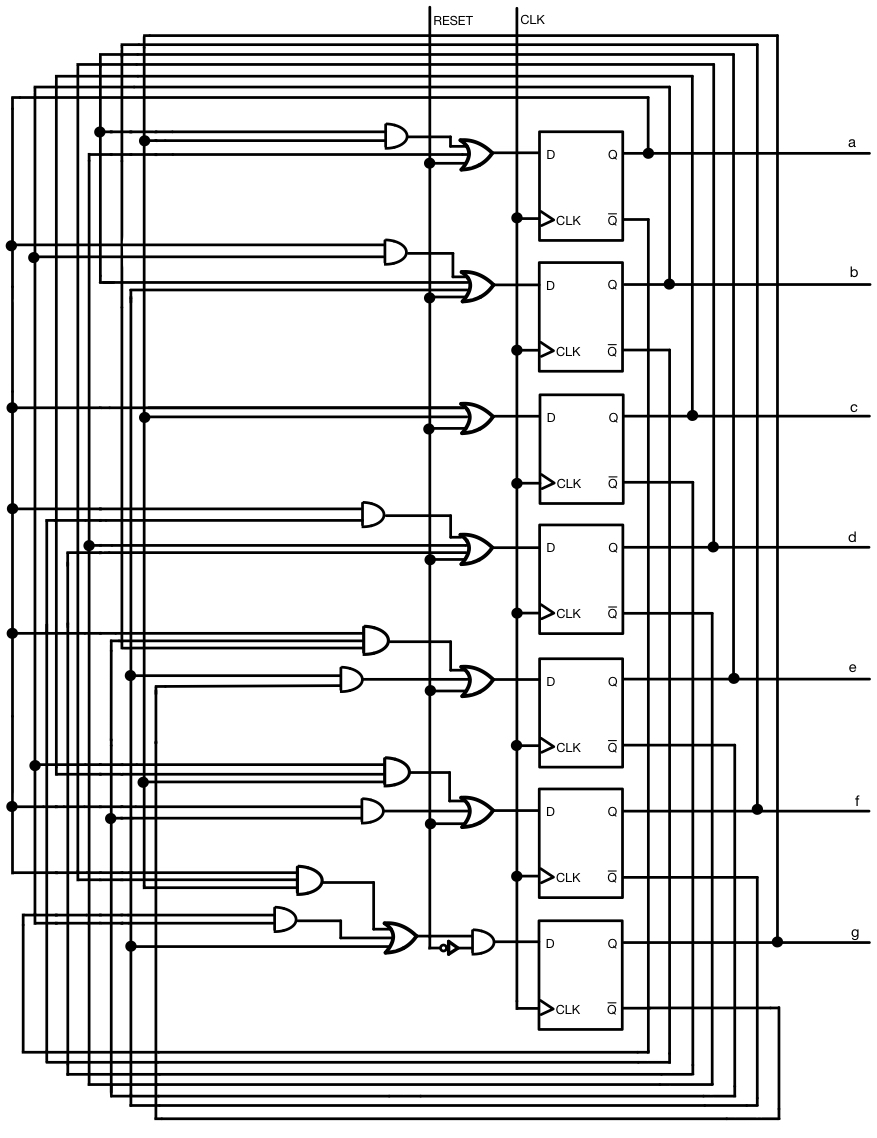
\includegraphics[width=\textwidth]{figs/p1.jpeg}
            \end{center}

        \item \textbf{Problem 2}: \emph{LFSR Design} \\
            In order to design the LFSR which will count every single 9 bit
            value, begin with the 9 bit LFSR that produces the maximum length
            sequence excluding zero. This is an LFSR using feedback bits 8, and
            4, so a sequence of DFFs in series with Q outputs from bits 4 and 8
            fed into an XOR gate which feeds the D input of the first DFF in the 
            series. 

            To include zero in the sequence of the LFSR, we must both force zero
            into the shift register, and out of zero. To do this, consider how
            we can force the register OUT of the all zero state. This is simple,
            essentially add a NOR gate on all of the Q outputs of the DFFs and 
            OR the result with the output of the XOR gate. This way, if the 
            LFSR is in the all zero state, the new gate will drive the input to
            the first DFF to 1, and the LFSR will begin its sequence from 
            0b100000000.
            
            To force the zero value into the LFSR, we need to be conscious of
            where in the sequence to insert 0. We would like to insert 0 into
            the output sequence right before the LFSR would output ob100000000,
            so that the sequence will be exactly the same as before with a zero
            inserted, but with a zero inserted. The value which would normally
            precede 0b100000000 is 0b000000001, since the 1 at bit 8 would drive
            the XOR gate high and result in shifting in a 1 to a register which
            is otherwise all 0. So to include 0, we need to force the transition
            from 0b000000001 to 0b000000000. This is simple. Only allow the XOR
            output to drive the first DFF high when bit 8 is not the only high 
            bit in the register. We are already checking for the all zero state
            with the NOR gate. Remove bit 8 from the AND gate and then XOR the
            output of the NOR gate with the output of the XOR gate. Now, if all
            signals other than bit 8 are low, the first XOR gate and the NOR
            both be high. Taking the XOR will result in a low signal, loading a
            0 into the first DFF so that the sequence will be 0b000000000. We
            still will be able to recover from the all zero state, since on the
            next clock cycle, the XOR will be low and the NOR will be high,
            meaning we will get the sequence 0b100000000 and jump back into the 
            normal sequence.

            This described LFSR is implemented in the following circuit, which
            will ouput the enumerated values on $I_8...I_0$:
            \begin{center}
                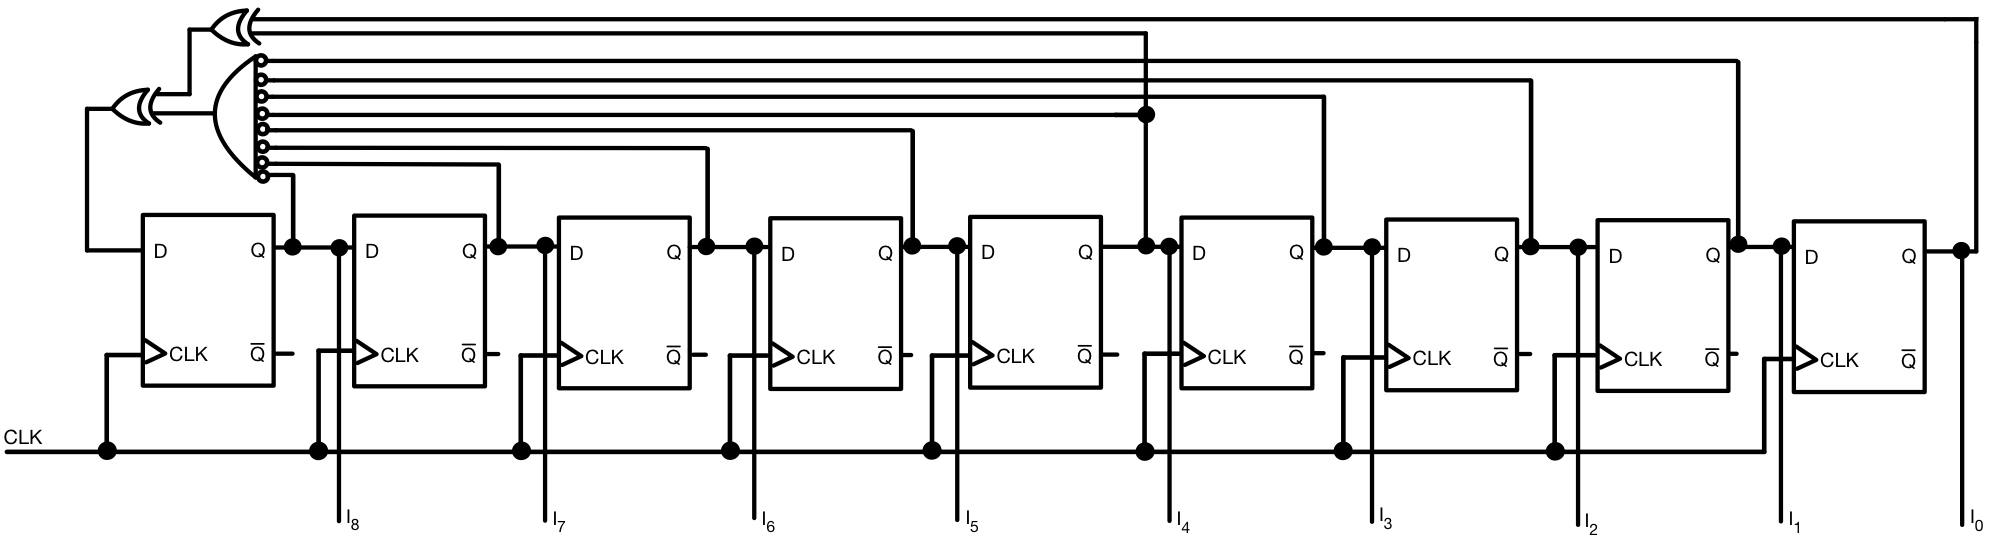
\includegraphics[width=\textwidth]{figs/p2.jpeg}
            \end{center}

            Notice that the gate count here is the count of the 9 DFFs, plus 10.
            This should be around 64 gates. Compare this to a 9 bit synchronous
            counter, which should require 1 DFF, 1 XOR gate, and 1 AND gate per
            bit, giving roughly 94 to 95 gates. This LFSR uses around 30 less
            gates, making it massively more efficient!
            \pagebreak

        \item \textbf{Problem 3}: \emph{Range Counter} \\
        
        The design for this problem is fairly simple. Begin by creating a
        standard 7 bit counter. This is a bunch of flip flops where each output
        is fedback through an XOR gate to its own input, and an AND gate to the
        next input. The result is that every bit is high if either all previous
        bits are high, or the bit is high and not all previous bits are high.

        We can simplify this a bit. Simply connect the D-input on bit 0 to its
        own $\overline{Q}$ output so that it toggles on every clock cycle. Then
        bit 6 also doesn't need to output to an AND gate since it we aren't
        prompted to include a carry out signal. 

        Now, we need to restrict the range and include the RESET signal. To
        detect the top end of the range, place an AND gate out the outputs which
        detects the exact top end of the range. We can ignore bit 5 since it will
        never be high concurrently with bit 6 given the range restriction. We
        need to force the circuit to output 8 if either this AND gate is high,
        or the reset signal is high. Therefore, feed the RESET signal and the
        output of the AND gate into an OR gate. Take the resulting signal and
        OR it with the logic on the D-input of bit 3 so that bit 3 will go high
        if the range tops out or if the reset signal is high. Then, negate the 
        output of the OR gate and AND the negation with all of the D-inputs of 
        the other bits. This way, if either RESET is high or the range tops out,
        only bit 3 will be high and we will get the desired output of 8.

        This results in the following set of equations:

        \begin{tabular}{|l|}
            \hline
            $R = I_6I_4I_3I_2'I_1'I_0 + RESET$ \\
            $I_0 = R'I_0'$ \\
            $I_1 = R'(I_0 \oplus I_1)$ \\
            $I_2 = R'(I_0I_1 \oplus I_2)$ \\
            $I_3 = R + (I_0I_1I_2 \oplus I_3)$ \\
            $I_4 = R'(I_0I_1I_2I_3 \oplus I_4)$ \\
            $I_5 = R'(I_0I_1I_2I_3I_4 \oplus I_5)$ \\
            $I_6 = R'(I_0I_2I_3I_4I_5 \oplus I_6)$ \\
            \hline
        \end{tabular}

        The resulting logic is implemented in the following circuit, which outputs
        the counter values on $I_6...I_0$:
        \begin{center}
            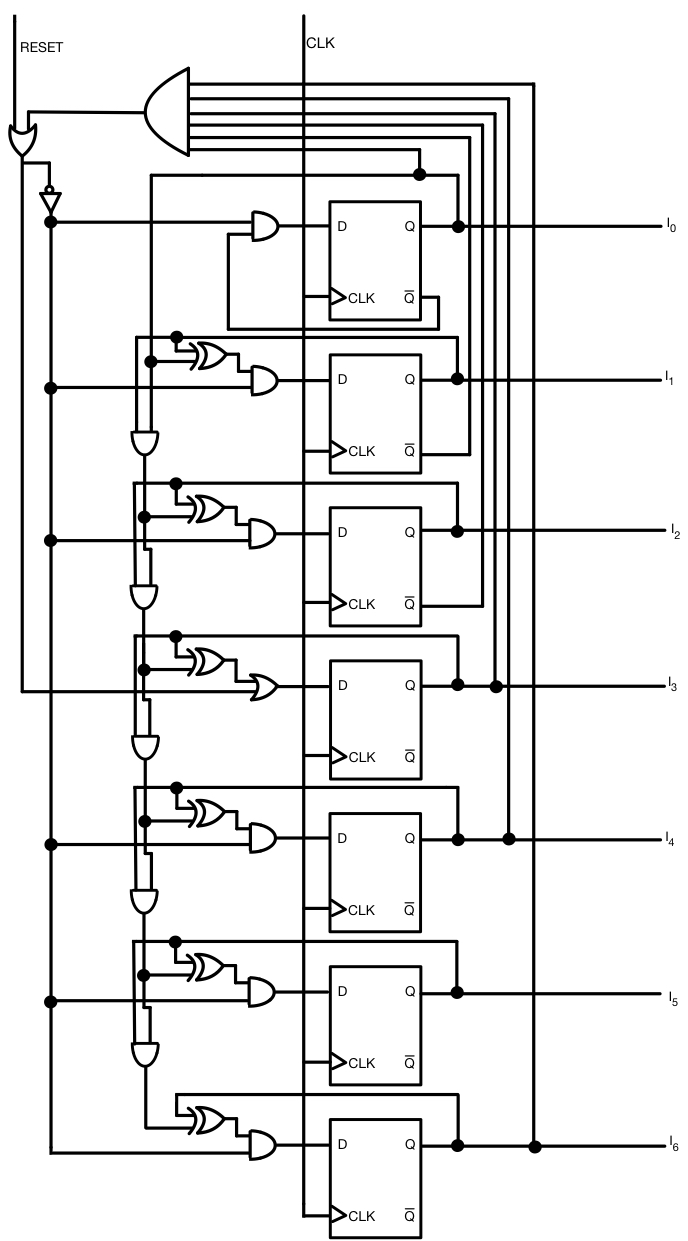
\includegraphics[width=0.75\textwidth]{figs/p3.jpeg}
        \end{center}

    \item \textbf{Problem 4}: \emph{Synchronous Design} \\
    
    To determine the rule violation of synchronous design rules, it is useful to
    enumerate the synchronous design rules. These are:

    \begin{enumerate}
        \item Use only D flip-flops are storage elements
        \item Non-synchronous presets and clear are not allowed (other than
              gglobal system reset)
        \item All DFFs need to be on the same global clock signal
        \item Sys clock may not be gated
        \item External and non-synchronous signals must be synchronized to the 
              clock.
    \end{enumerate}

    The violations of these rules that occur within the Craps game design are as 
    follows: 

    \begin{enumerate}
        \item Packages U1 and U5 are 74LS92 counters. These counters use 
              JK flip-flops as storage elements, which are not D flip-flops, and
              therefore violate rule a listed above. 
        \item The system clock signal is gated by part U18C on the way into U1,
              violating rule d listed above.
        \item Part U7 is a 74LS175 containing 4DFFS. However its clock signal 
              is connected to combinational logic, not the system clock line,
              unlike its counterpart DFFs in U8 which are on the clock generated
              by X1. This violates rule c listed above.
        \item Roll is an external signal generated off of switch S1, which is 
              not synchronized to the system clock. This violates rule e listed 
              above.
    \end{enumerate}


    \end{enumerate}

    \pagebreak
    \begin{scriptsize}
    \verbatiminput{../Q-M/qm.py}
    \pagebreak
    \verbatiminput{p1.py}
    \end{scriptsize}

\end{document}
